%%%%%%%%%%%%%%%%%%%%%%%%%%%%%%%%%%%%%%%%%%%%%%%%%%%%%%%%%%%%%%%%%%%%%%%%
%Created 2011-09-22 Thu 14:51
\documentclass[11pt]{article}
%\documentclass[11pt]{standalone}

\usepackage{dingbat}  %% for \checkmark
\usepackage{lipsum,pdflscape}
\usepackage{blindtext}
\usepackage{scrextend}
\addtokomafont{labelinglabel}{\sffamily}

\usepackage[table]{xcolor}
\usepackage{colortbl}

\usepackage{fourier} 
\usepackage{array}
\usepackage{makecell}

%\renewcommand\theadalign{bc}
%\renewcommand\theadfont{\bfseries}
%\renewcommand\theadgape{\Gape[4pt]}
%\renewcommand\cellgape{\Gape[4pt]}

\usepackage[hyphens]{url}
\usepackage{graphicx}
\usepackage{longtable}
\usepackage{wrapfig}
\usepackage{soul}
\usepackage{marvosym}
\usepackage{wasysym}
\usepackage{latexsym}
\usepackage{amssymb}
\usepackage{array}
\input pro_preamble.tex

\usepackage{natbib}
\usepackage{verbatim}
\usepackage{afterpage}
\usepackage{lipsum}
\usepackage{authblk}
\usepackage[vertfit]{breakurl}
\usepackage[nottoc,numbib]{tocbibind}

\usepackage{tikz}
\usetikzlibrary{shapes, arrows}

\usepackage{fancyhdr}
\pagestyle{fancy}
\fancyhf{} % clear all fields
\headheight=30pt
\headsep=5pt
\lhead{}
\rhead{}
\cfoot{\thepage}

\newcommand{\degree}{\ensuremath{^\circ \;}}
\newcommand{\kc}{\textsf{kCARTA}\xspace}
\newcommand{\sa}{\textsf{SARTA}\xspace}
\newcommand{\sasc}{\textsf{SARTA-TwoSlab}\xspace}
\newcommand{\pcrtm}{\textsf{PCRTM}\xspace}
\newcommand{\disort}{\textsf{DISORT}\xspace}
\newcommand{\ecmwfXsarta}{\textsf{ecmwf2sarta}\xspace}
\newcommand{\ecmwf}{\textsf{ECMWF}\xspace}
%\newcommand{\eg}{\textit{e.g.}\xspace}
%\setcounter{section}{-1}


%%%%%%%%%%%%%%%%%%%%%%%%%
%% https://tex.stackexchange.com/questions/124605/section-title-coloring-code-makes-table-of-content-numbered
%% this is supposedly better, notice EXPLICIT written there
\usepackage{xcolor,lipsum}
\usepackage[explicit]{titlesec}

%% can use \eg {gray!10} as above or \eg {blue!05} etc
\titleformat{name=\section}[block]
  {\sffamily\large}
  {}
  {0pt}
  {\colorbox{blue!10}{\parbox{\dimexpr\textwidth-2\fboxsep}{\strut\thesection~#1\strut}}}
\titleformat{name=\section,numberless}[block]
  {\sffamily\large}
  {}
  {0pt}
  {\colorbox{blue!10}{\parbox{\dimexpr\textwidth-2\fboxsep}{\strut#1\strut}}}
\titlespacing*{\section}{0pt}{\baselineskip}{\baselineskip}


%%%%%%%%%%%%%%%%%%%%%%%%%

\titlespacing*{\section}
{0pt}{1.0ex}{1.0ex}
\titlespacing*{\subsection}
{0pt}{1.0ex}{1.0ex}

\providecommand{\alert}[1]{\textbf{#1}}

\usepackage{enumitem}   %% for lists
\setlist{leftmargin=5.5mm}
\setlist[enumerate]{itemindent=\dimexpr\labelwidth+\labelsep\relax,leftmargin=0pt}

\setlength{\textfloatsep}{-0.1cm}

\begin{document}

%\setlength{\parindent}{22em}

%%%%% REMOVE THIS IN FINAL VERSION
%% \begin{comment}

\renewcommand\thepage{}
\newpage
\renewcommand\thepage{\arabic{page}}

%\label{sec-1}

\setcounter{page}{1}

% https://www.purdue.edu/business/sps/pdf/NASA_Proposal_Preperation.pdf
% https://nspires.nasaprs.com/tutorials/PDF_Guidelines.pdf
% https://smd-prod.s3.amazonaws.com/science-red/s3fs-public/atoms/files/PSD_DMP_Template_v4.txt

%\title{NNH23ZDA010L : Single Footprint Thermodynamic and Cloud Retrievals}
\title{SARTA ANALYTIC JACOBIANS}
\author{Sergio DeSouza-Machado$^{1}$ and Larrabee Strow$^{1,2}$}
\affil{\vspace{-0.1in} \small{$^{1}$ Joint Center For Earth Systems Technology, University of Maryland Baltimore County}}
\affil{\vspace{-0.1in} \small{$^{2}$ Department of Physics, University of Maryland Baltimore County  \\ contact : sergio@umbc.edu}}

\date{}

\maketitle

\vspace{-0.375in}
\pagenumbering{arabic}

\section{Introduction}

\sa is a fast Radiative Transfer code with TwoSlab Cloud scattering
ability \citep{mac:17*2} that has been extensively tested for clear
sky accuracy against \eg \kc \citep{mac:19} and clouds
\citep{mac:17*2,aum:18,aum:23}.

It currently takes about 4 minutes to generate radiances for one
granule of AIRS L1C data (2645 channels $\times$ 12150 FOVS), given
input atmospheric profiles (thermodynamic and cloud) supplied by \eg
radiosondes or Numerical Weather Prediction (NWP) model fields that are put into a 
100 layer atmosphere model.

This is more than adequate for processing observations for comparison
purposes (given that line by line codes such as \kc take about 40
seconds to process one spectrum!). But if used for retrievals where
estimates of jacobians are needed, the times become very large (for
example would need to run it 100 times for T(z) jacobians, 100 times
for WV(z) jacobians and another 100 times for O3(z) jacobians, or
about 20 hours for all channels; more if you need \eg CH4, N2o etc
jacobians).

For these purposes, an analytic \sa jacobian code has been
written. This document outlines the changes to the \sa code, and the
ideas behind propagating the thermodynamic (temperature and
constituent gases) analytic derivatives at layer $j$ to the Top of
Atmosphere (TOA); cloud jacobians still need to be done by finite
difference.

\section{\sa original flow}

Figure \ref{fig:fig1} shows the ``regular'' \sa flow diagram. After
opening an rtp file and reading in the 7 sets of coefficients, it then
generates all the predictors for each of the 7 breakout sets
(ycalparX, $X=1,7$) and then produces the ODs for all 7 sets
  (ycaltX\_od, $X=1,7$). After that it loops over each required channel
    to do the radiative transfer, pulling in the necessary ODs for the
    ycaltX\_od as needed.  We remind the reader the scattering
    radiative transfer is a weighted sum over 4 radiance streams :
    clear, cloud 1 only,cloud2 only and cloud1,2

\begin{figure}[ht] \centering
   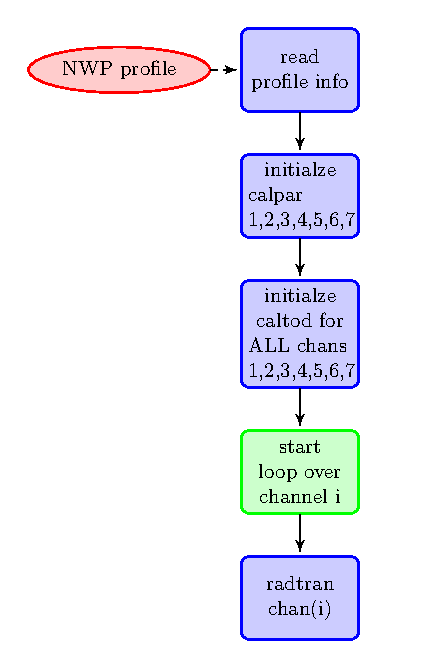
\includegraphics[width=.75\textwidth]{sarta_diagram1.pdf}
\caption{Flow diagram of \sa PGE etc}
\label{fig:fig1}
\end{figure}

\section{\sa analytic jacobian flow}

Figure \ref{fig:fig2} shows the ``analytic jacobian'' \sa flow diagram. The main difference is that
the loops over channels start at the (ycaltX\_od(i), $X=1,7$), continuing 
with the radiative transfer.

\begin{figure}[ht] \centering
   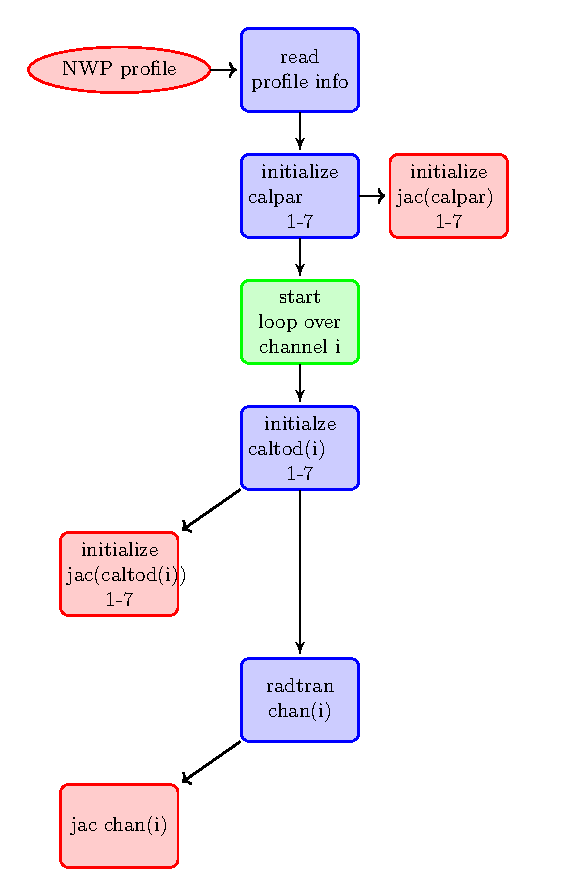
\includegraphics[width=.75\textwidth]{sarta_diagram2.pdf}
\caption{Flow diagram of \sa Analytic Jacobian}
\label{fig:fig2}
\end{figure}

\section{The Analytic Derivatives of the Predictors}

The SARTA clear sky details are encapsulated in \eg \citep{str:02*2}
where based on coefficients $C_j$ and predictors $P_j$ based on the
atmospheric profiles and view angles \textit{T(z), WV(z), O3(z), sec($\theta$)}
so one can form effective optical depths at each layer L
\[
\tau(i,L) = \sum_{j=1}^J C_{j} P_{j}(T(z),WV(z),O3(z),\theta)
\]
with $J$ typically being less than 10; the ODs are computed \textit{at each layer L = 1,100}
(where $L=1$ = TOA and $L=N$ is GND) for \eg variable gases WV, CO2,
O3, N2O, CO, CH4, SO2, HNO3 and the ``rest of the uniform fixed
gases'' which include O2, N2 etc, using the atmospheric profiles \textit{T(z),WV(z),O3(z)} and
view angle information $\theta$.

This formulation makes it evident that the jacobian is `''simply''
related to the derivative of $\tau$ with respect to any thermodynamic
variable $X$ (where $X$ can be temperature, water vapor amount, ozone
amount, etc), given by
\begin{equation}
\frac{\partial \tau(i,L)}{\partial X_L} = \sum_{j=1}^J C_{j} \frac{\partial P_{j}(T(z),WV(z),O3(z),sec(\theta))}{\partial X_L}
\label{eqn:deriv}
\end{equation}
and so can ``easily'' be calculated, using the same coefficients
$C(j)$. \textit{Note these derivatives are for optical depth at angle
  $\theta$ }

\subsection{``Simply'' the derivative}

We will typically denote the $T,WV,O3$ derivatives as
\textit{\_T,\_1,\_3}.  Most of the predictors simply depend on layer
$L$, and the derivatives of $P(L)$ can indeed be obtained very simply by using
the product rule, for example as seen in Table \ref{table:table1}

%\begin{landscape}
\begin{table}[htbp]
\footnotesize
\begin{tabular}{ccccc}
PREDICTOR NAME  & THERMODYNAMIC            & $\frac{\partial P}{\partial T_l}$ & $\frac{\partial P}{\partial WV_l}$ & $\frac{\partial P}{\partial O3_l}$ \\
\textit{P(L)}   &  + CONSTITUENT           &      P(L)\_T                     &        P(L)\_1                      & P(L)\_3 \\
                &  DEPENDENCE              &                                  &                                     & \\ 
\hline
    TR          &     T(L)/TREF(L)         & $\frac{1}{TREF(L)}$              &              0                   & 0 \\ 
    DT          &    PTEMP(L) - RTEMP(L)   &      1                           &              0                   & 0 \\
    A\_W        &    PWAMNT(L)/RWAMNT(L)   &      0                           & 1/RWAMNT(L)                      & 0 \\
    A\_O        &    POAMNT(L)/ROAMNT(L)   &      0                           & 0                                & 1/ROAMNT(L) \\
    TJUNKS      &          TR*TR           &    2*TR*TR\_T                    & 0                                & 0 \\
    FPRED1(1)   & SECANG(L)*TJUNKS         & SECANG(L)*TJUNKS\_T              & 0                                & 0 \\
    OPRED1(3)   & SECANG(L)*A\_O*DT        & SECANG(L)*A\_O*DT\_T             & 0                                & SECANG(L)*DT*A\_O\_3 \\
                &                          & = SECANG(L)*A\_O                 &                                  & = SECANG(L)*DT/ROAMNT(L)\\    
\hline
\end{tabular}
\caption{Easy derivatives}
\label{table:table1}
\end{table}
%\end{landscape}

\subsection{Not so ``Simply'' the derivative}
Of course things are not always so simple. This is especially so in
the case of the predictor depending on ``all the layers above layer
L'' $P(L,L-1,L-2,...1)$, with layer $L=1$ being the TOA. For example
\[
\begin{array}{ccc}
PDP(L)   & = & PRES(L) (PRES(L)-PRES(L-1))    \\
WZREF(L) & = & \sum_{j=1}^L PDP(J) WAMNT(J)^{ref} \\
WZ(L)    & = & \sum_{j=1}^L PDP(J) WAMNT(J)       \\
AZ\_W(L) & = & \frac{WZ(L)}{WZREF(L)}         \\
\end{array}
\]

So technically if you perturb layer $L$ you also ``perturb'' all
layers above it. Which means if the amount of water vapor in layer $L$
is increased by $\alpha$, so is that of all the layers above it $WZ(L)
\rightarrow WZ(L)(1 + \alpha)$, while of course the reference
amount(s) stay unchanged. This means the original amounts (denoted by ``0'' below)

\[
AZ\_W0(L) = \frac{WZ0(L)}{WZREF(L)} = \frac{\sum_{j=1}^L PDP(j) WAMNT(j)}{\sum_{j=1}^L PDP(j) WAMNT(j)^{ref}} 
\]

are changed to amounts X below

\[
AZ\_WX(L) = \frac{WZX(L)}{WZREF(L)} = \frac{\sum_{j=1}^L PDP(j) WAMNT(j) (1 + \alpha)}{\sum_{j=1}^L PDP(j) WAMNT(j)^{ref}} 
\]

and so the change in $AZ\_W(L)$ which is the cumulative amount at layer $L$ is now 
\[
\begin{array}{ccc}
\frac{\Delta(AZ\_W(L))}{\Delta(Gas Amount(L))} &  = & \frac{AZ\_WX(L) - AZ\_W0(L)}{\alpha  WAMNT(L)} \\
                                               & =  & \frac{\alpha  \sum PDP(j) WAMNT(j)}{\sum PDP(j) WAMNT(j)^{ref}}  \frac{1}{\alpha  WAMNT(L)} \\
\frac{\partial AZ\_W(L)}{\partial WAMNT(L)}    & =  & \frac{AZ\_W(L)}{WAMNT(L)} \\
\end{array}
\]

We can now use these ideas to get the derivatives of the `predictors
which depend on these `layer above'' predictors! for example as seen
in Table \ref{table:table2}

%\begin{landscape}
\begin{table}[htbp]
\footnotesize
\begin{tabular}{ccccc}
PREDICTOR NAME  & THERMODYNAMIC            & $\frac{\partial P}{\partial T_l}$ & $\frac{\partial P}{\partial WV_l}$ & $\frac{\partial P}{\partial O3_l}$ \\
\textit{P(L)}   &  + CONSTITUENT           &      P(L)\_T                     &        P(L)\_1                      & P(L)\_3 \\
                &  DEPENDENCE              &                                  &                                     & \\ 
\hline
    A\_W        &    PWAMNT(L)/RWAMNT(L)   & 0            & 1/RWAMNT(L)                                             & 0 \\
    WJUNKA      &    SECANG(L)*A\_W        & 0            &  SECANG(L)*A\_W\_1                                      & 0 \\
    WJUNKZ      &    WJUNKA*A\_W/AZ\_W     & 0            &  WJUNKA\_1*A\_W/AZ\_W +                                 & 0 \\ 
                &                          &              & WJUNKA*(AZ\_W*A\_W\_1 - A\_W*AZ\_W\_1)/AZ\_W/AZ\_W      & \\
\hline
\end{tabular}
\caption{Not so Easy derivatives}
\label{table:table2}
\end{table}
%\end{landscape}

\subsection{OPTRAN}

The above coefficients and predictors are based on a pressure scale
(ie given index $L$ you always know the pressure $P(L)$; it is the gas
amount $Q(L)$ and temperature $T(L)$ which must be given to you by \eg
a sonde measurement or a NWP model, in order for you to estimate the
gas optical depth $OD(L) = OD(q(L),T(L),p(L)) = OD(q(L(p)),T(L(p)))$
ie temperature and gas amounts are predictors.

The gas amounts and mixing ratios of variable gases such as WV vary by
orders of magnitude over the 0-80 km of a typical atmosphere
model. The OPTRAN \citep{mcm:95*1} methodology estimates optical
depths using layer to space gas amount as the grid, with pressure
being a predictor $OD(L) = OD(Q(A),T(A),p(A)) = OD(T(A(a)),P(A(a)))$
ie temperature and pressures are predictors. SO one has to interpolate
$p,T$ and the weighted $p,T$ onto these grids, do the OPTRAN fast
model coefficient $\times$ predictor magic, then interpolate back ont
other usual AIRS 100 layers pressure grid.

Which means the jacobians need to involve all these stages
... complicating things quite a bit.  But the ideas remain the same;
some are simple derivatives, most are ``layer above''
derivatives. Once they are computed, they need to be used in
differentiating the linear weighting terms that put the P(L) onto the
A(a) grid.  Once that is done, the optical depths need to be
interpolated onto the layer-to-space absorption grid; so once again
the derivatives need to be computed there. Quite a mess.

\section{Propagating analytic derivatives from layer $j$ to TOA}

The one layer clear sky equation governing radiative transfer (\citep{mac:19,goo:89,lio:80}) is given by 
\begin{equation}
\mu(\theta) \frac{d r(\nu)}{d \tau_0} = -r(\nu) + B(\nu,T)
\label{eqn:eqn1}
\end{equation}

where $\mu$ is the cosine of the zenith angle $\theta$, $B(T)$ is the
Planck function at layer temperature $T$ and $r(\nu)$ is the Planck
radiance at wavenumber $\nu$. Finally $\tau_0$ is the nadir optical
depth; the optical depth at angle $\theta$ is given by
\begin{equation}
\tau(\theta) = \frac{\tau_0}{cos(\theta)} = \frac{1}{\mu} \tau_0 
\label{eqn:eqn2}
\end{equation}

At the top of layer $i$, the solution to is
\begin{equation}
r_i(\nu) = r_{i-1}(\nu) e^{-\frac{\tau_{0}(i,\nu)}{\mu}} + B(\nu,T_i) (1 - e^{-\frac{\tau_{0}(i,\nu)}{\mu}})
\label{eqn:eqn3}
\end{equation}
where $r_{i-1}$ is the radiation incident at the bottom of this layer
from the top of the previous layer $i-1$ (or if $i=1$, the surface
emission $\epsilon(\nu) B(\nu,T_S)$).

Propagating this up through many layers $N$ then gives the radiance at the TOA

\begin{equation}
r_{N} = \epsilon(\nu) B(\nu,T_S) e^{-\sum_i=1^N \frac{\tau_{0}(i,\nu)}{\mu}} + \sum_i^N B(\nu,T_i) (1 - e^{-\frac{\tau_{0}(i,\nu)}{\mu}}) e^{-\sum_{j=i+1}^N \frac{\tau_{0}(j,\nu)}{\mu}}
\label{eqn:eqn4}
\end{equation}

\subsection{Derivatives for one layer}

We are interested in temperature and gas constituent derivatives for a
clear sky; Remember optical depth depends on gas amount $q$ and
temperature $T$ (since layer $i$ implicitly also gives a pressure
dependence); Then for one layer we can differentiate Equation \ref{eqn:eqn3}
with respect to temperature $T$ and gas amount $q$ to get (after some
algebra, and dropping layer index $i$ and wavenumber dependence $\nu$
from the equations)

\begin{equation}
\frac{\partial r}{\partial T} = \left( \mu \frac{\partial r}{\partial \tau_0} \right) \left( \frac{1}{\mu} \frac{\partial \tau_0}{\partial T} \right) + \frac{\partial B(T)}{\partial T} (1 - e^{\frac{\tau_0}{\mu}}) = A(r) E(T) + C(T)
\label{eqn:eqn1T}
\end{equation}

\begin{equation}
\frac{\partial r}{\partial q} = \left( \mu \frac{\partial r}{\partial \tau_0} \right) \left(   \frac{1}{\mu} \frac{\partial \tau_0}{\partial q} \right)  = A(r) G(q)
\label{eqn:eqn1Q}
\end{equation}

Looks complicated but we know everything (also see \eg Equation 8 in \citep{liu:06}) : 
\begin{itemize}
\item the radiance derivatives wrt OD $A(r) =  \mu \frac{\partial r}{\partial \tau_0} $ from the right hand side of Equation \ref{eqn:eqn1} above
\item the right hand side of Equation \ref{eqn:eqn3} above says what top-of-layer radiance to use in $A(r)$
\item the OD partial derivatives wrt thermodynamic variables $E(T) =  \frac{1}{\mu} \frac{\partial \tau_0}{\partial T} , G(q) =  \frac{1}{\mu} \frac{\partial \tau_0}{\partial q} $ come from Equation \ref{eqn:deriv} above!
\item it is trivial to compute $C(T) = \frac{\partial B(T)}{\partial T} (1 - e^{\frac{\tau_0}{\mu}})$
\end{itemize}

\subsection{Derivatives for one layer at TOA}

But you need to propagate it up! Remember the radiative transfer is
done iteratively, or if you like recursively; since the radiation from
surface goes through layer 1, then to layer 2 and so on till layer N
at TOA. Which means

\begin{equation}
r_N(\nu) = r_{N-1}(\nu) e^{-\frac{\tau_{0}(N,\nu)}{\mu}} + B(\nu,T_N) (1 - e^{-\frac{\tau_{0}(N,\nu)}{\mu}})
%\label{eqn:eqnN}
\end{equation}

But since
\begin{equation}
r_{N-1}(\nu) = r_{N-2}(\nu) e^{-\frac{\tau_{0}(N-1,\nu)}{\mu}} + B(\nu,T_{N-1}) (1 - e^{-\frac{\tau_{0}(N-1,\nu)}{\mu}})
%\label{eqn:eqnN-1}
\end{equation}

that means 
\begin{equation}
r_N(\nu) = r_{N-1}(\nu,r_{N_2}(\nu)) e^{-\frac{\tau_{0}(N,\nu)}{\mu}} + B(\nu,T_N) (1 - e^{-\frac{\tau_{0}(N,\nu)}{\mu}})
%\label{eqn:eqnNN}
\end{equation}

and so on to the layer you are interested in $J$
\begin{equation}
r_N(\nu) = r_{N-1}(\nu,r_{N_2}(\nu,r_{N_2}(\nu(....(r_{J}(\nu,T_j,q_j)))))) e^{-\frac{\tau_{0}(N,\nu)}{\mu}} + B(\nu,T_N) (1 - e^{-\frac{\tau_{0}(N,\nu)}{\mu}})
\label{eqn:eqnNJ}
\end{equation}

Recall that radiances at the bottom of layer $i$ are attenuated by
$e^{-{\tau_{0}(i,\nu)}{\mu}}$ as they propagate to the top of the
layer. This means differentiating Equation \ref{eqn:eqnNJ} gives an
attenuation from every layer above that ie from the top of the layer $J$ to the TOA

\begin{equation}
\frac{\partial r_{N}}{\partial X_{J}} = \frac{\partial r_{N}}{\partial r_{N-1}}  \frac{\partial r_{N-1}}{\partial r_{N-2}} \frac{\partial r_{N-2}}{\partial r_{N-3}} ... \frac{\partial r_{J+1}}{\partial r_{J}} \frac{\partial r_{J}}{\partial X_{J}}
\end{equation}
\begin{equation}
\frac{\partial r_{N}}{\partial X_{J}} = e^{-\frac{\tau_{0}(N,\nu)}{\mu}} e^{-\frac{\tau_{0}(N-1,\nu)}{\mu}} e^{-\frac{\tau_{0}(N-2,\nu)}{\mu}} ... e^{-\frac{\tau_{0}(J+1,\nu)}{\mu}} \frac{\partial r_{J}}{\partial X_{J}}
\end{equation}
\begin{equation}
\frac{\partial r_{N}}{\partial X_{J}} = e^{-\sum_{k=J+1}^N \frac{\tau_{0}(k,\nu)}{\mu}} \frac{\partial r_{J}}{\partial X_{J}}
\end{equation}

where we know $\frac{\partial r_{J}}{\partial X_{J}}$ from the one layer derivatives in Equations \ref{eqn:eqn1T},\ref{eqn:eqn1Q} above! Again, also See Equation 8 in \citep{liu:06}!!!

\section{Various : surface and background thermal and solar contribution and NLTE}

\subsection{Surface}
The surface emission term, seen at TOA, is given by
\[
r_{surface}(\nu) = \epsilon(\nu) B(\nu,T_S) e^{-\sum_1^N \frac{\tau_0(\nu,i)}{\mu}}
\]
which means the derivative at the TOA is given by 
\[
\frac{\partial r_{surface}(\nu)}{\partial T_s} = \epsilon(\nu) \frac{\partial B(\nu,T_S)}{\partial T} e^{-\sum_1^N \frac{\tau_0(\nu,i)}{\mu}}
\]

\subsection{Background thermal}
This is technically complicated, but lets assume we have calculated
the term propagating downwards and have it as $r_{background}(\nu)$
just as it is incident downwards at the surface. It is then reflected
and propagates to the TOA, attenuated at each layer as it goes up. So
the term at the TOA is 
\[
r_{reflected\_thermal(\nu)} = \rho(\nu) r_{background}(\nu) e^{-\sum_1^N \frac{\tau_0(\nu,i)}{\mu}}
\]
where typically $\rho(\nu) = (1-\epsilon(\nu))/\pi$ (Lambertian
reflectance). The derivatives at each layer are then added on to the jacobians above, given by
\[
\frac{\partial r_{reflected\_thermal(\nu)}}{\partial X_J} = -\frac{1}{\mu} \tau_0(\nu,J) \frac{\partial \tau_0(\nu,J)}{\partial X_J}r_{reflected\_thermal(\nu)}
\]

\subsection{Solar}
This is technically complicated, but lets assume we have calculated
the solar term propagating downwards and have it as $r_{solar}(\nu)$
just as it is incident downwards at the surface. It is then reflected
and propagates to the TOA, attenuated at each layer as it goes up. So
the term at the TOA is 
\[
r_{reflected\_solar(\nu)} = \rho(\nu) r_{solar}(\nu,\theta_{sun}) e^{-\sum_1^N \frac{\tau_0(\nu,i)}{\mu}}
\]
where typically $\rho(\nu) = (1-\epsilon(\nu))/\pi$ (Lambertian
reflectance). The derivatives at each layer are then added on to the jacobians above, given by
\[
\frac{\partial r_{reflected\_solar(\nu)}}{\partial X_J} = -\frac{1}{\mu} \tau_0(\nu,J) \frac{\partial \tau_0(\nu,J)}{\partial X_J}r_{reflected\_solar(\nu)}
\]
Note we have assume $\rho(\nu)$ is the same for reflected thermal and
for reflected solar; this is not necessarily correct as eg sun glint
would be almost mirror like.

\subsection{NLTE}
There is a correction term to the 4.3 um radiance due to NLTE
in the upper atmosphere. It currently depends only on the temperature
of the top 5 layers, the satzen and solzen angles, and \cd gas amount
(or more accurately, deviation from 385 ppm). This is modeled as
\[
\delta r_{NLTE}(\nu) = (\sum_j^6 N_j(\nu) NLTE\_PRED(j)) (N_7 (co2ppm-385)+1)
\]
The temperature dependence is only in predictor 5 $via$ NLTE\_PRED5 = 1/5(T1+T2+T3+T4+T5), so 

\[
\frac{\partial \delta r_{NLTE}(\nu)}{\partial T_i} = N_5 (0.2) (1) (N_7 (co2ppm-385)+1), i=1,2,3,4,5
\]

and can be trivially added on; similarly the \cd gas amount jacobian can be done but it is tiny (at least over about 50 ppmv changes).

\section{Two slab clouds : weighted sum over four radiance streams}

We use the PCLSAM parametrization for clouds and aerosols in \sa and
\kc (see \citep{mac:17*2,mac:19}). Here the cloud scattering effects
are re-parametrized into an effective optical depth. It's not as
accurate as \eg DISORT \citep{stam:88} but its fast and simple, and the
accuracy can be improved \citep{tang:18}. All this means our final
radiation is
\begin{itemize}
\item a weighted sum over clear, cloud1 fraction, cloud 2 fraction, cloud 1+2 overlap
\item more importantly, clouds 1 and 2 go into our atmosphere
  effectively as two additional non-scattering ``gases''; so their
  effects can be added in as an additional ``fixed'' gas.
\end{itemize}

All the above equations remain fundamentally unchanged, except we \eg
increase the total OD of layer(s) $i1$ by that of cloud 1, and the
total OD of layer(s) $i2$ by that of cloud 2, while doing the cloud1
only, cloud 2 only, and cloud 1+2 portions of the radiative transfer.

Then jacobians in our TwoSlab atmosphere, are simply done as above,
but for each of the four streams; and then just as final radiance is
the weighted sum of the four radiance streams, the final jacobian is
the weighted sum of the four jacobians.

The rtp file allows us to have the following variables :
(ctype1,cfrac1,cngwat1,csze1,cprtop1,
cprbot1),(ctype2,cfrac2,cngwat2,csze2,cprtop2,
cprbot2),(cfrac12). Based on these, assuming all the fractions are
non-zero the code then defines \textit{cx1 = c1 - c12, cx2 = c2 - c12, fclr = 1 - (c1x+c2x+c12) = 1 - (c1+c2-c12)}

Then we find the radiance as 
\begin{small}
\[
\begin{array}{ccccccccc}
r(\nu) & = & fclr \;\;\; rclr(\nu)           & + & c1x \;\;\; r1(\nu)      & + & c2x \;\;\; r2(\nu)      & + & c12 \;\;\; r12(\nu) \\
       & = & (1-(c1+c2-c12)) \;\;\; rclr(\nu) & + & (c1-c12) \;\;\; r1(\nu) & + & (c2-c12) \;\;\; r2(\nu) & + & c12 \;\;\; r12(\nu) \\
\end{array}
\]
\end{small}

The PCLSAM effective nadir cloud optical depth \citep{cho:99} is given by
\begin{eqnarray*}
 \tau_{cld}(\nu,sze,cng,\theta = 0) & = & cng \times \left( \tau^{1g/m2}_{ext}(\nu,sze) - \frac{1}{2}\tau^{1g/m2}_{sca}(\nu,sze)(1 + g(\nu,sze)) \right) \\
                              & = & cng \times \tau^{1g/m2}(\nu,sze,\theta = 0) \\
                              & = & cng \times f(\nu,sze) \\
\end{eqnarray*}

where $cng$ is the cloud loading in g/m2, $sze$ is effective particle
diameter in um, $g(\nu)$ is the asymmetry and $\omega =
\tau_{sca}(\nu)/\tau_{ext}(\nu) =
(\tau_{ext}(\nu)-\tau_{abs}(\nu))/\tau_{ext}(\nu)$.  The superscript
$1g/m2$ means everything has been saved/normalized to this cloud
loading.

This means for example 
\begin{enumerate}
\item the nadir cloud optical depth is related to cloud optical depth at angle $\theta$ by
\begin{eqnarray*}
 \tau_{cld}(\nu,sze,cng,\theta) & = & \frac{1}{cos(\theta)} \tau_{cld}(\nu,sze,\theta = 0) \\
                          & = & \frac{1}{\mu} \tau_{cld}(\nu,sze,\theta = 0) \\
\end{eqnarray*}

\item the derivative with respect to cloud amount (ignoring angles) is trivially
\begin{eqnarray*}
\frac{\partial \tau_{cld}}{\partial cng} & = & \frac{\tau_{cld}(\nu)}{cng} \\
                                   & = & \tau^{1g/m2}(\nu,sze,\theta = 0) = f(\nu,sze) \\
\end{eqnarray*}

\item the derivative with respect to cloud particle size is
\begin{eqnarray*}
\frac{\partial \tau_{cld}}{\partial sze} & = & cng \times  \left( \frac{\partial \tau^{1g/m2}_{ext}(\nu,sze)}{\partial dze} \right) - \\
                                         &   & \frac{cng}{2} \left( \frac{\partial \tau^{1g/m2}_{sca}(\nu,sze)}{\partial dze} (1 + g(\nu,sze)) \right) - \\
                                         &   & \frac{cng}{2}  \left(  \tau^{1g/m2}_{sca}(\nu,sze) \frac{\partial g(\nu,sze)}{\partial sze}) \right) \\
                                         & = & cng \frac{\partial f}{\partial sze} \\
\end{eqnarray*}

\item furthermore suppose the cloud is defined between $cprtop$ mb and
  $cprbot$ mb. Then it typically straddles more than one layer. The
  (cloud loading $cng$) fraction in each layer $L$ that the cloud
  straddles is given by (exept at top most/bottom most cloud layer)
\[
  frc_{cng}(L) = \frac{plev(L+1)-plev(L)}{cprtop-cprbot}, LCLDTOP \le L \le LCLDBOT
\]

so that each layer has fraction $frc_{cng}(L)
\tau_{cld}(\nu,sze,\theta)$ of the total cloud optical depth. The
derivatives of $frc_{cng}(L)$ with respect to $cprtop,cprbot$ are
trivially (which of course means its not so trivial and the jacs are awful)

\[
\frac{\partial frc_{cng}(L)}{\partial cprtop} = (-1) \frac{plev(L+1)-plev(L)}{(cprtop-cprbot)^2} \times (+1);
\frac{\partial frc_{cng}(L)}{\partial cprbot} = (-1) \frac{plev(L+1)-plev(L)}{(cprtop-cprbot)^2} \times (-1);
\]

(\textcolor{red}{though compared to \sa finite differences, the
  $cprtop,cprbot$ derivatives are sometimes off by -1 ... but this is
  probably due to finite difference perturbation in pressure ensuring
  cloud top/bottom layer is slightly different}.

\item This partitioning of the total cloud OD into the individual AIRS
  pressure layers according to $frc_{cng}(L)$ has couple of
  implications for the jacobians : for any one of the four streams
  (clear, cloud1, cloud2, cloud1+2), 
  \begin{itemize}

  \item to get the \textit{cpsize,cngwat} column jacobian, we sum over
    each of the cloud layers (from LCTOP to LCBOT) with the layer
    contribution weighted by $frc_{cng}(L)$.

  \item to get the \textit{cprtop,cprbot} parameters we need the the
    $frc_{cng}(L)$ changes at each layer, and so to get the column
    sum, \textit{we weight each layer by 1}

  \end{itemize}
\end{enumerate}

\subsection{Cloud Fraction jacs}
From above, the jacobians wrt cloud fraction (ie a unity change!! pretty large!!!) are immediately
\[
\begin{array}{ccc}
\frac{\partial r(\nu)}{\partial c1} & = & -rclr(\nu) + r1(\nu) \\
\frac{\partial r(\nu)}{\partial c2} & = & -rclr(\nu) + r2(\nu) \\
\frac{\partial r(\nu)}{\partial c12} & = & +rclr(\nu) - r1(\nu) - r2(\nu) + r12(\nu) \\
\end{array}
\]

\subsection{Cloud Amount and Cloud Particle Size jacs}

As mentioned above our look-up tables are in terms of $\tau_{cld}(\nu) = cldOD(\nu) = cng \;\;\; f(\nu,sze)$ from which (and use the formulation above)
\[
\begin{array}{ccc}
\hline
cldOD(\nu) & = & cng \;\;\; f(\nu,sze) \\
\hline
\frac{\partial cldOD}{\partial sze} & = & cng \frac{\partial f(\nu,sze)}{\partial sze} \\
\frac{\partial r(\nu)}{\partial sze1} & = & \frac{\partial r1(\nu)}{\partial sze1} + \frac{\partial r12(\nu)}{\partial sze1} \\
                                      & = & \frac{\partial r1(\nu,sze)}{\partial cldOD1} \frac{\partial cldOD1}{\partial sze1} + \frac{\partial r12(\nu)} {\partial cldOD1} \frac{\partial cldOD1}{\partial sze1} \\
                                      & = & cng1 \left(\frac{\partial r1(\nu,sze)}{\partial cldOD1} \frac{\partial f1(\nu,sze1)}{\partial sze1} + \frac{\partial r12(\nu)} {\partial cldOD1} \frac{\partial f1(\nu,sze1)}{\partial sze1} \right) \\
\frac{\partial r(\nu)}{\partial sze2} & = & \frac{\partial r2(\nu)}{\partial sze2} + \frac{\partial r12(\nu)}{\partial sze2} \\
                                      & = & \frac{\partial r2(\nu,sze)}{\partial cldOD2} \frac{\partial cldOD2}{\partial sze2} + \frac{\partial r12(\nu)} {\partial cldOD2} \frac{\partial cldOD2}{\partial sze2} \\
                                      & = & cng2 \left(\frac{\partial r2(\nu,sze)}{\partial cldOD2} \frac{\partial f2(\nu,sze2)}{\partial sze2} + \frac{\partial r12(\nu)} {\partial cldOD2} \frac{\partial f2(\nu,sze2)}{\partial sze2} \right) \\
\hline
\frac{\partial cldOD}{\partial cng} & = & f(\nu,sze) \\
\frac{\partial r(\nu)}{\partial cng1} & = & \frac{\partial r1(\nu)}{\partial cng1} + \frac{\partial r12(\nu)}{\partial cng1} \\
                                      & = & \frac{\partial r1(\nu,cng)}{\partial cldOD1} \frac{\partial cldOD1}{\partial cng1} + \frac{\partial r12(\nu)} {\partial cldOD1} \frac{\partial cldOD1}{\partial cng1} \\
                                      & = & \frac{\partial r1(\nu,cng)}{\partial cldOD1} f1(\nu,cng1) + \frac{\partial r12(\nu)} {\partial cldOD1} f1(\nu,sze1) \\
\frac{\partial r(\nu)}{\partial cng2} & = & \frac{\partial r2(\nu)}{\partial cng2} + \frac{\partial r12(\nu)}{\partial cng2} \\
                                      & = & \frac{\partial r2(\nu,cng)}{\partial cldOD2} \frac{\partial cldOD2}{\partial cng2} + \frac{\partial r12(\nu)} {\partial cldOD2} \frac{\partial cldOD2}{\partial cng2} \\
                                      & = & \frac{\partial r2(\nu,cng)}{\partial cldOD2} f2(\nu,cng2) + \frac{\partial r12(\nu)} {\partial cldOD2} f2(\nu,sze2) \\
\end{array}
\]

\subsection{Cloud Top and Cloud Bottom jacs}

Scott has a cool way of implementing the cloud
boundaries across pressure level boundaries and so can occupy a
fraction of an AIRS layer; \kc ``fills'' in AIRS pressure levels so
the cloud occupies one or more \textit{full} pressure layers; all the
cloud jacobian stuff I do for single footprint retrievals, ensure that
(a) cld1 bottom and cld2 top do not merge/overlap (b) cld1 top or cld2 top
does not become less than 0 mb (c) cld1 bottom or cld2 bottom does not
become more than surf pres. But I did make a stab at it!!! Recall for any layer $L$ the total optical depth is given by 

\begin{eqnarray*}
\tau_{total}(T,q_1,q_2,q_3,....,q_{fixed},cld_1,cld_2) & = & \tau_1(T,q_1) + \tau_2(T,q_2) + .... \tau_{12}(T,q_{12}) + \\
                                                       &   & \tau_{cld1}(cng1,sze1,cprtop1,cprbot1,species1) + \\
                                                       &   & \tau_{cld2}(cng2,sze2,cprtop2,cprbot2,species2) \\
\end{eqnarray*}
which means (assuming variable we are interested in $X_i$ is not the temperature $T$)
\[ 
\frac{\partial \tau_{total}}{\partial X_i} = \frac{\partial \tau_{i}}{\partial X_i}, i=q_1,q_2,....q_{12},cld1 params, cld2 params
\]

From above, we have cloud loading fractions $frc_{cng}(L)$ and their derivatives, so in layer $L$
\begin{eqnarray*}
\frac{\partial r(\nu,L)}{\partial cprtop/bot}  & = &  \frac{\partial r(\nu,L)}{\partial \tau_{total}(\nu)} \frac{\partial \tau_{total}(\nu)}{\partial cprtop/bot} \\
\frac{\partial r(\nu,L)}{\partial cprtop/bot}  & = &  \frac{\partial r(\nu,L)}{\partial \tau_{total}(\nu)} \frac{\partial \tau_{cld}(\nu)}{\partial cprtop/bot} \\
\frac{\partial r(\nu,L)}{\partial cprtop/bot}  & = &  \left( \mu \frac{\partial r(\nu,L)}{\partial \tau_{total}(\nu)} \right) \left( \frac{1}{\mu} \frac{\partial \tau_{cld}(\nu)}{\partial cprtop/bot} \right) \\
\frac{\partial r(\nu,L)}{\partial cprtop/bot}  & = &  \left( -r_L + B_L \right) \left( \frac{1}{\mu} \frac{\partial \tau_{cld}(\nu)}{\partial cprtop/bot} \right) \\
\end{eqnarray*}

We know 
\[
\tau_{cld}(\nu,L) = frc_{cng}(L) \tau^{total}_{cld}(\nu) =  frc_{cng}(L) cng \times  \tau^{1g/m2}(\nu,sze,\theta = 0)
\]
which means
\begin{eqnarray*}
\frac{\partial \tau_{cld}(\nu)}{\partial frc_{cng}(L)} & = & cng \times  \tau^{1g/m2}(\nu,sze,\theta = 0) \\
\frac{\partial \tau_{cld}(\nu)}{\partial cprtop}       & = & \frac{\partial \tau_{cld}(\nu)}{\partial frc_{cng}(L)} \frac{\partial frc_{cng}(L)}{\partial cprtop} \\
%                                                       & = & \left. \frac{\partial \tau_{cld}(\nu)}{\partial frc_{cng}(L)}\right/ \frac{\partial cprtop}{\partial frc_{cng}(L)} \\
\frac{\partial \tau_{cld}(\nu)}{\partial cprbot}       & = & \frac{\partial \tau_{cld}(\nu)}{\partial frc_{cng}(L)} \frac{\partial frc_{cng}(L)}{\partial cprbot} \\
%                                                       & = & \left. \frac{\partial \tau_{cld}(\nu)}{\partial frc_{cng}(L)} \right/ \frac{\partial cprbot}{\partial frc_{cng}(L)} \\
\end{eqnarray*}

and then we can use the same formulation as for $T(z),G1(z),...$ etc
derivatives!! 

\section{Running SARTA Analytic Jacobian}

This is very similar to running \sa as usual, except there are couple
additional command line arguments, and you read in the output
jacobians using Matlab. A typical run would be \newline

\begin{verbatim}
  [name of exec] fin=blah.op.rtp fout=blah.rad.rtp               RADS ONLY
  [name of exec] fin=blah.op.rtp fout=blah.rad.rtp listj=-1      RADS and JACS
\end{verbatim}

\subsection{Command Line arguments}

Command line arguments include what Scott had \eg ``rhot'' with a
couple new important ones; run times change appropriately as you
change any or all of num of chans/jacs/profiles

\begin{itemize}
\item   listp = list of profiles [Scott had this]
  \begin{itemize}
  \item listp allows you to choose upto 20 profiles (default -1 = all, or just
  leave out this arg)
  \end{itemize}  
\item   listc = list of channels [new]
  \begin{itemize}
  \item listc allows you to choose upto 20 channel IDs \eg 1291 for the 1231
  cm=1, or 449 for 791 cm-1. (default -1 = all, or just leave out this arg)
  \end{itemize}
\item   listj = list of jacobians [new]
  \begin{itemize}
  \item If you leave out listj, it does NO jacobians (ie radiance calcs) default

  \item If you want jacs, then listj = -1 gives WGT, T, GID 1,2,3,4,5,6,9,12
                                or listj = your list \eg 300,100,1,2,3    would give CLD, T and GID 1,2,3
  \end{itemize}
\end{itemize}

\section{Output readers}
Right now the default is to change $\frac{\partial
  r(\nu,TOA)}{\partial T_J}$, $\frac{\partial r(\nu,TOA)}{\partial
  Q_J}$, $\frac{\partial r(\nu,TOA)}{\partial CLD_J}$ to
$\frac{\partial BT(\nu,TOA)}{\partial T_J}$, $\frac{Q_J \partial
  BT(\nu,TOA)}{\partial Q_J}$, $\frac{CLD_J \partial
  BT(\nu,TOA)}{\partial CLD_J}$ but this can easily be coded out. The
output jac files (f77 binary files) would have root name of fout,
followed by \_jacT or \_jacGX or \_jacCLD appended to them

\begin{verbatim}
Reader : /home/sergio/KCARTA/MATLAB/
[w,d,iaProf,iaNumLay] = readsarta\_jac(fname,type)
  eg.   'newdayx.rtp_WGTFCN',200  would read in weight functions
        'newdayx,rtp_jacTZ',100                 temp jacs 
        'newdayx.rtp_jacG1,',1                  G1 jacs etc

For G1,G2, ... jacs (and weight functions) d would, for example, be
    24x2645x100    (24 profiles, 2645 channels, 100 layers)
For T          jacs, d would, for example, be
    24x2645x101    (24 profiles, 2645 channels, 100 layers+surface temp)
For Cloud      jacs, d would, for example, be
    24x2645x012    (24 profiles, 2645 channels, 12 jacs)
    01-05 : [cfrac1,cngwat1,cpsize1,cprtop1,cprbot1],
    06-10 : [cfrac2,cngwat2,cpsize2,cprtop2,cprbot2],
    11    : cfrac12
    12    : stemp 

while if you do
  [h,ha,p,pa] = rtpread('blah.rad.rtp');
then $w = h.vchan$ (ie the $h.vchan$ from the output radiance file)
\end{verbatim} 

iaProf lists the profiles you asked to calculate jacs for (from listp
above), while iaNumLay is basically (for WGT FCN and gas jacs)
p.nlevs-1 for those profiles, and an extra one for stemp for temp jacs
(so has length p.nlevs)

\section{The End (sort of)}

Finite difference \sa jacobians agree with kCARTA analytic jacobians
except in the window region, since \kc needs the cloud top and bottoms
to be at pressure level boundaries, full cloud layers while \sa allows
the top and bottom pressures to be ``anywhere''. 

The \sa analytic jacobians have been compared to \sa finite difference
jacobians, and kCARTA analytic jacobians. The agreement is very good,
except sometimes the \textit{cprtop or cprbot} derivatives can be
flipped by a sign since the finite difference jacobian straddles (or
loses) an additional cloud layer.

Figure \ref{fig:fig3} shows a typical comparison of \sa analytic
versus \sa finite difference column jacobians.

\begin{figure}[ht] \centering
   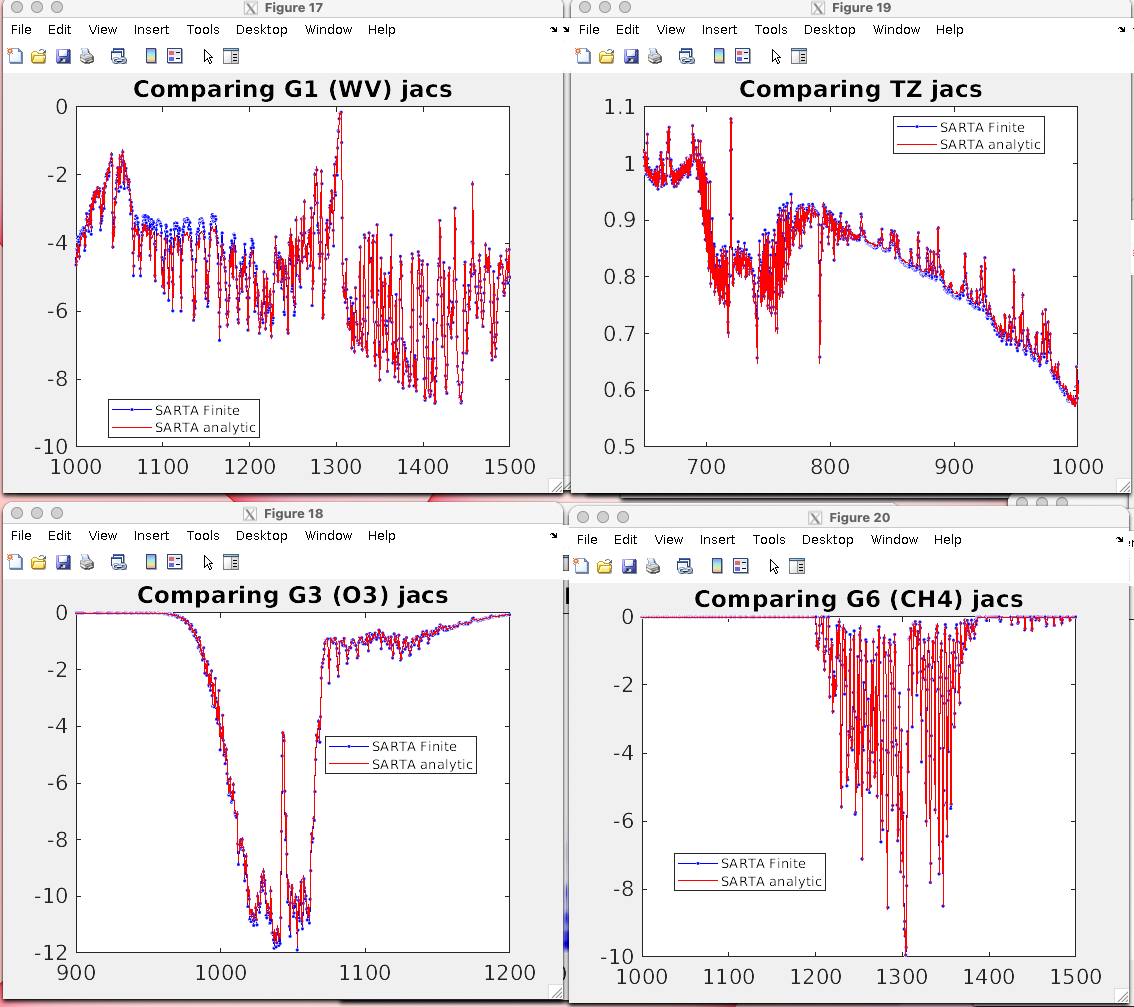
\includegraphics[width=.75\textwidth]{compare_finite_diff.png}
\caption{Comparison of \sa finite diff VS analytic column jacobians}
\label{fig:fig3}
\end{figure}

Feel free to test and give feedback. Its a mix of old f77 \sa code
(the June 20, 2022 commit) first rewritten to loop over ichan) and
then jacobians with f90 implicit loops. No modules (yet, dunno if
ever). I assume if the incFTC link is changed to CRIS or IASI and the
code re-compiled, it should work (there are about 2-3 extra parameters
in the current file, mostly jacobian matrix size). And fingers crossed
you keep breakouts/predictors the same ie never ever change the bloody
predictors.  You can compare to finite diff jacs, done for only your
chosen profile, using /home/sergio/MATLABCODE\_Git/quicksartajac.m
(make sure the finite diff jacobians use eg dQ=0.01 or dT = 0.1, else
the numerical noise will creep in and ratios of jacs will look awful).
The testing code wrappers which call both the finite difference
jacobian code, and the analytic jacobian code, are in the MATLABCODE
subdirectory, and have the names 
\begin{verbatim} test_jac_AIRS.m, test_jac_CRIS.m,test_jac_IASI.m 
\end{verbatim}
The results are of comparing eg
$\sum(TZ_{finite}(i=1:100))/\sum(TZ_{analytic}(i=1:100))$ and
$\sum(G1_{finite}(i=1:100))/\sum(G1_{analytic}(i=1:100))$ etc should all
be very close to one and should lie on top of each other; similarly
the cloud jacobians shoul all lie close to each other.

Run times for 12150 profiles/2645 AIRS channels is 4 minutes, while
adding in all jacobians and weighting functions (T jacs,
G1,2,3,4,5,6,9,12 jacs) increases the run time by $\times$ 10. This is
compared to running \sa over and over for about 10 extra
perturbations $\times$ 100 layers to get the corresponding finite
difference jacobians, which is about 66 hours or about 2.75 days.

\section{Acknowledgment}
Scott Hannon wrote/developed most of the original \sa code with
Larrabee Strow and Howard Motteler. He worked closely with me on the
interfacing with TwoSlab clouds. Tobias Wehr wrote parts of a HIRS
Fast model analytic code and put that into a write up, which inspired
me to do this! Seeing Xu Liu's expressions for PCRTM derivatives are a
confirmation that I was on the right track in ``propagating the
derivatives''.

\bibliographystyle{plainnat}
\bibliography{/home/sergio/texmf/bibtex/bib/atmspec2017}

\end{document}
